\section{AutoSynch: An Automatic-Signal Monitor Based on Predicate tagging \\ 
\small{Wei-Lun Hung, Vigay K. Garag}}

\subsection{notes}

This paper aims to automate signaling around thread access to shared objects in
Java. The key idea is that signaling requires expertise and a lot of code, but
it is really the same code each time. The authors build a library Autosynch,
which signals waiting threads when predicates become true automaticly,
eliminating the need for thread specific signaling, and reducing the number of
blunt calls to \emph{SignalAll()}.

The meat of this paper, and a lot of the key insights seem to come from the
evaluation of local predicates. The key challange is that from the perspective
of a global moniter, local variables are invisable. Evaluating predicates composed of only global variables is trivial (according to the paper).

The authors make an interesting observation, about the performance of checking
predicates on the fly. They tag predicates in order to check them when values
change. Where some predicate $P = c_0 \wedge c_1 \wedge \dots \wedge c_n$. They
only tage the first conjunction $c_0$. The reasoning behind this is that all
conjunctions needto be true, so whenever any of them change it would be a good
reason to evaluate the predicate, except that it causes overhead. The idea is
check only when a single predicate changes, and hope that the rest are too. It
reduces the checking overhead by a lot I imagine.

They use an interesting heap structure to optimize signaling and checking.
Essentially they order threashold tags into a heap of equivilance ie $x < 5$ is
checked before $x < 7$ for unsigned ints because the space is smaller.
Aparantly this improves the speed of search. If I want to implement something
like this the heap may be key to getting good performance.

After working through the eval it seems clear that the real benifit to this
work is the simplicity of code, while still retaining performance. In most
cases they have to drive the number of threads up into the hundreds before they
see a performance win.

\subsection{observations}

Local predicates can be evaluated by treating their runtime values as constant.
The moment that the \textit{AutoSynch.WaitUntill($P$)} is executed and $P$
contains some local variables $L$ all variables $v \in L$ have their values
logged so the predicate can be evaluated globally.

The key insight to this paper is really that given a set of predicates, the
problem of issuing a signal to a waiting thread is as simple as finding a
waiting thread, not issuing signals to all. This approach requires a
centralized approach to issuing locks.


\begin{figure}[t]
    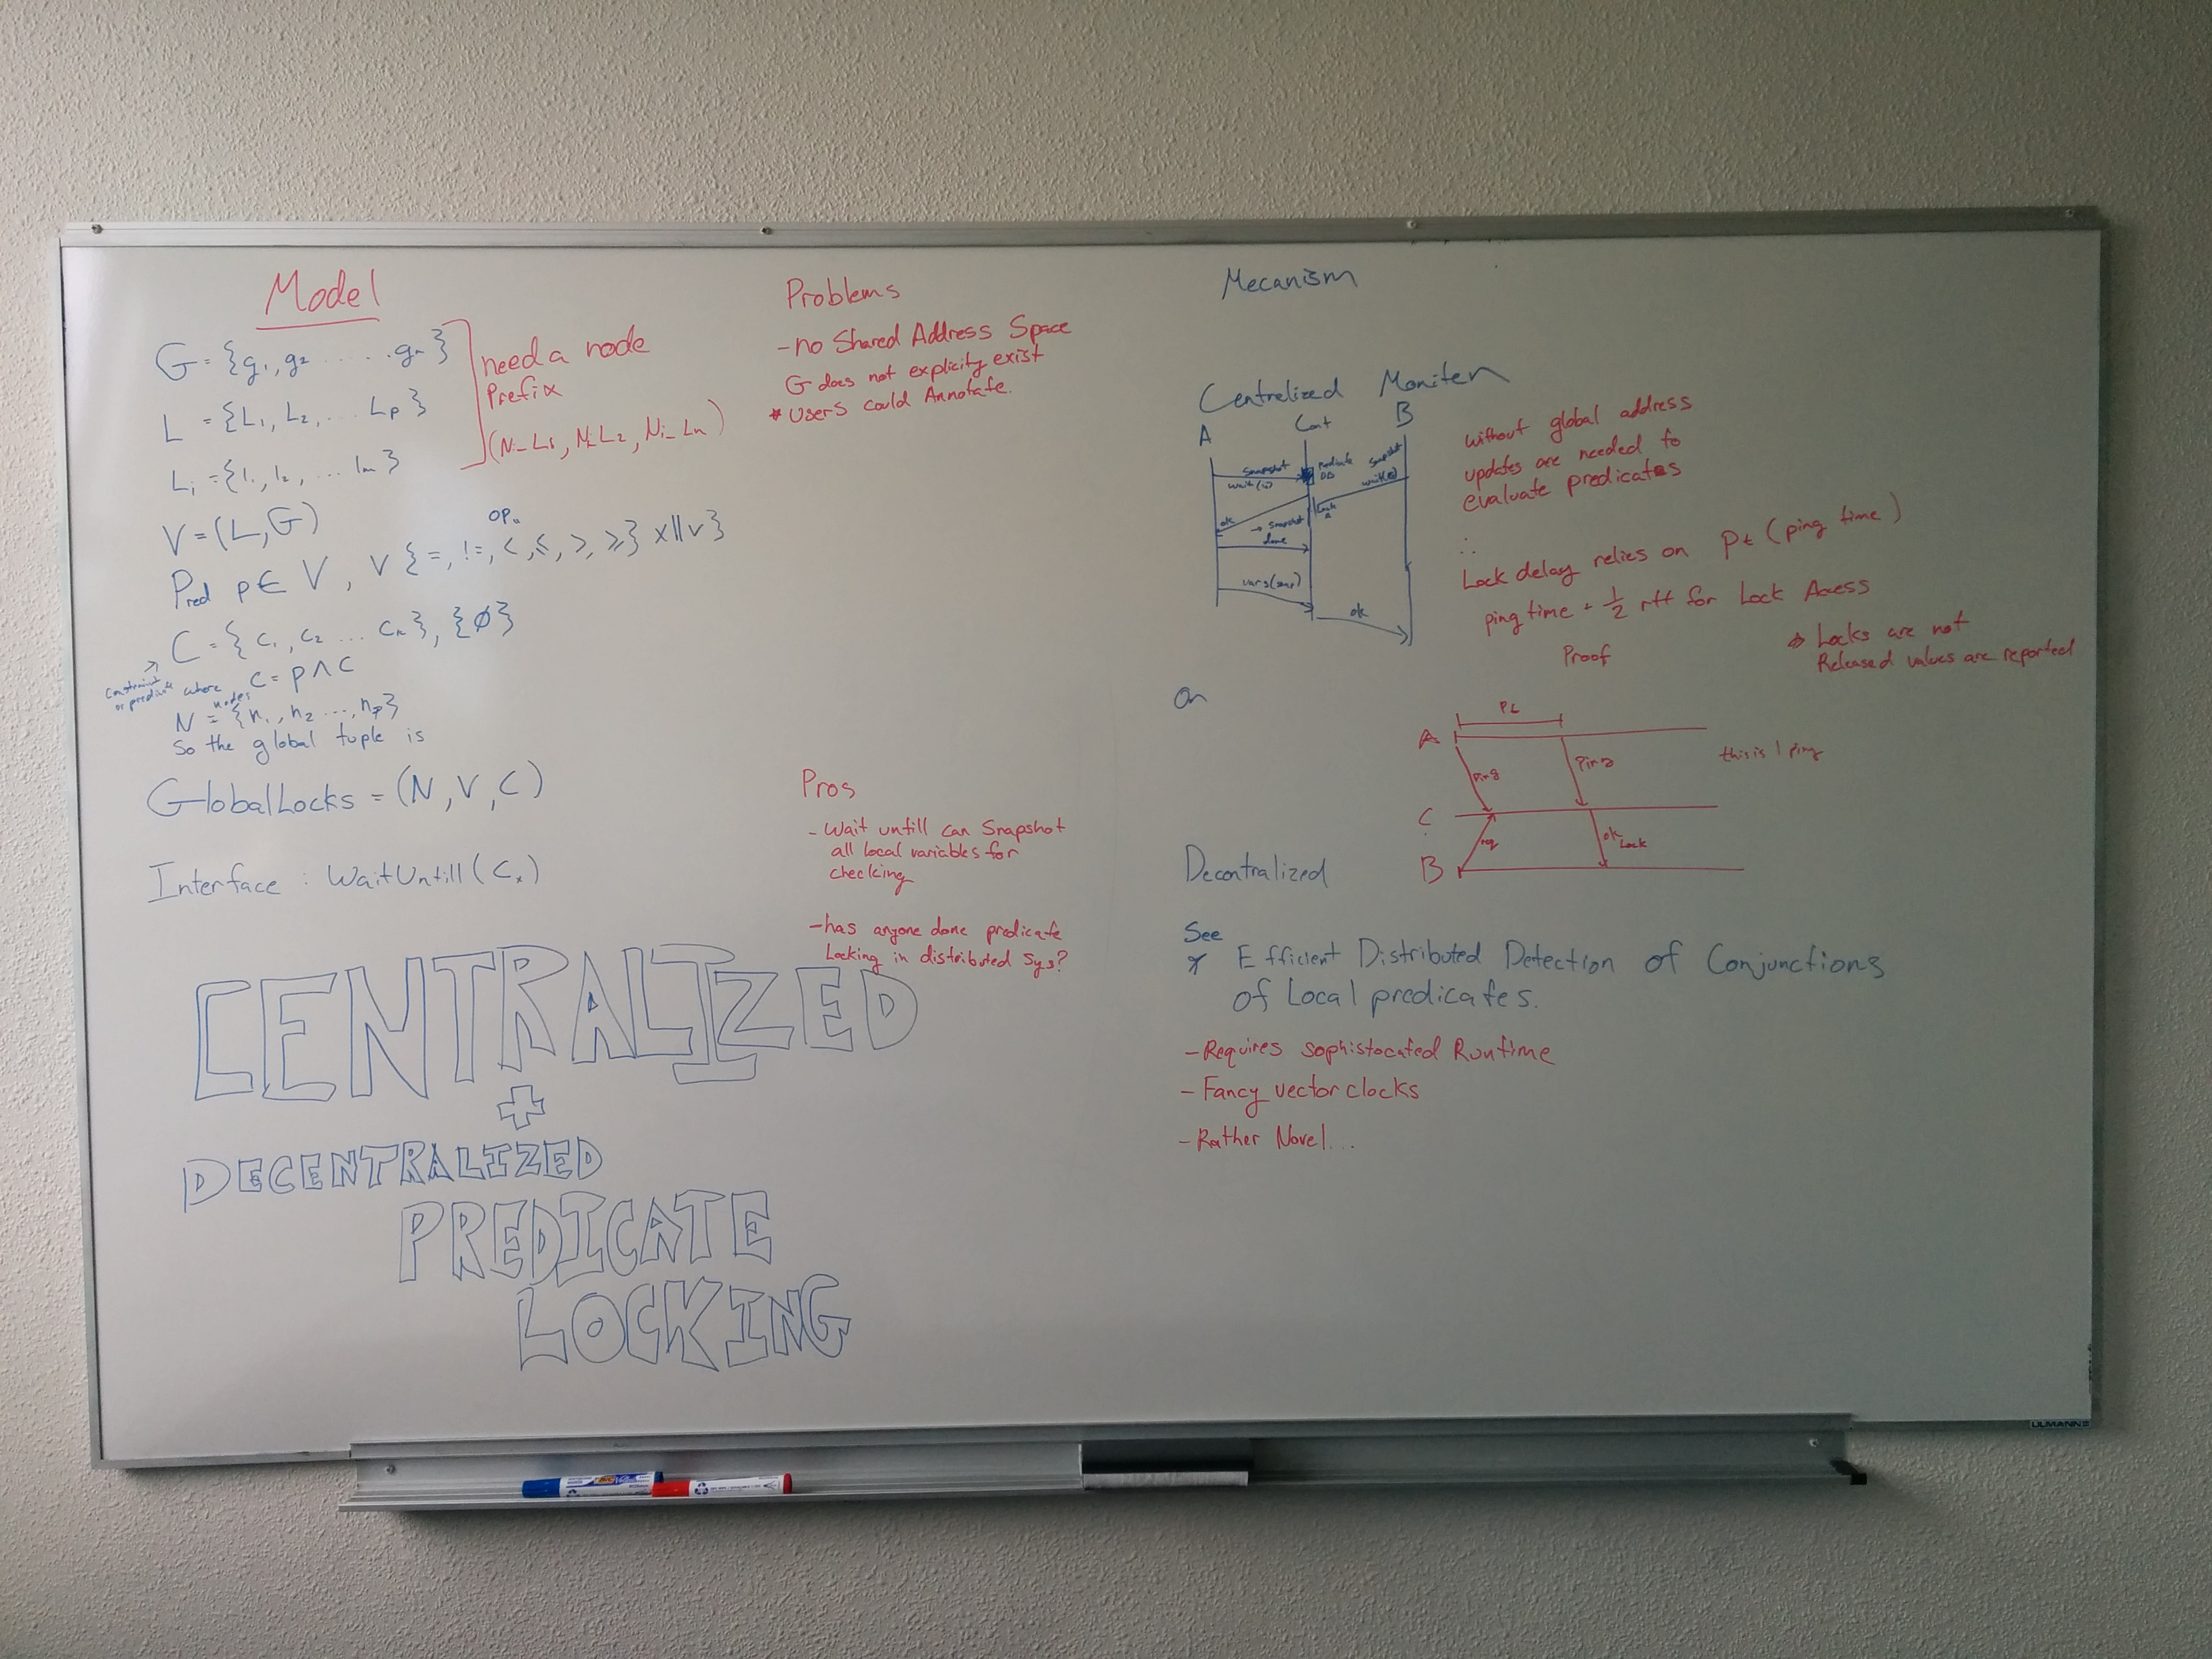
\includegraphics[width=0.50\textwidth]{fig/predicatelock}

    \caption{Whiteboard of potential distributed (centralized and
    decentralized) predicate locking}

\label{fig:espace} 
\end{figure}

\subsection{questions}

\begin{itemize}

    \item How do decentralized lock servers deal with fine grained locking such
as this. In the case of chubby the expection was that locks would last a long
time~\cite{Burrows:2006:CLS:1298455.1298487}. Has work been done where only
waiting threads are issued signals based on predicate evaluation, and not just
locks?

    \item Can the evaluation of predicated be done without a centralized source, and in an online fashion?

\end{itemize}


